% LTeX: enabled=false
% chktex-file 1
% chktex-file 8
% chktex-file 12
% chktex-file 15
% chktex-file 36
% chktex-file 46
% VLDB template version of 2020-08-03 enhances the ACM template, version 1.7.0:
% https://www.acm.org/publications/proceedings-template
% The ACM Latex guide provides further information about the ACM template

\documentclass[sigconf, pdfa, nonacm]{acmart}
\usepackage{subcaption}
\usepackage{algorithm}
\usepackage{algpseudocode}
\usepackage{listings}
\usepackage{balance}
\usepackage{microtype} % Improves spacing
\usepackage{booktabs}
\usepackage[a-2b]{pdfx} % Targets PDF/A-2b compliance
\hbadness=10000 % Suppresses underfull hbox warnings
\vbadness=10000 % Suppresses underfull vbox warnings

% \usepackage{enumitem}
% \setlist[itemize]{leftmargin=*, noitemsep, topsep=0pt}

\lstdefinestyle{query}{
    basicstyle=\footnotesize\ttfamily,
    frame=single,
    breaklines=true,
    language=SQL
}

\newenvironment{queryblock}{
    \renewcommand{\lstlistingname}{Query} % Changes caption prefix from 'Listing' to 'Query'
    \lstset{style=query}                   % Applies your custom query style
    \begin{figure}[htbp]           % Prevents page breaks within this block
}{
    \end{figure}
}

\newcommand\summary[1]{\paragraph{\textbf{#1}}}
\usepackage{tikz}
\usetikzlibrary{positioning}
\usetikzlibrary{shapes}
\usetikzlibrary{shapes.multipart}
%% The following content must be adapted for the final version
% paper-specific
\newcommand\vldbdoi{XX.XX/XXX.XX}
\newcommand\vldbpages{XXX-XXX}
% issue-specific
\newcommand\vldbvolume{19}
\newcommand\vldbissue{XX}
\newcommand\vldbyear{2026}
% should be fine as it is
\newcommand\vldbauthors{\authors}
\newcommand\vldbtitle{\shorttitle}
% leave empty if no availability url should be set
\newcommand\vldbavailabilityurl{https://github.com/alicia-lyu/vldb19-artifact}
% whether page numbers should be shown or not, use 'plain' for review versions, 'empty' for camera ready
\newcommand\vldbpagestyle{plain}


\begin{document}
\title{Storing and Indexing Multiple Tables by Interesting Orderings}
\subtitle{For Efficient Joins, Groupings, and Updates in Relational Databases}

\author{Wenhui Lyu} \orcid{0009-0008-0946-4414}
\affiliation{\institution{University of Wisconsin--Madison}} \email{wenhui@cs.wisc.edu}

\author{Goetz Graefe} \orcid{0000-0003-0194-6466}
\affiliation{\institution{Google Inc.}} \email{goetzg@google.com}
% LTeX: enabled=true


\begin{abstract}
Relational database systems face a fundamental tension between supporting multi-table queries and frequent updates. Materialized join views can drastically speed up queries, but they slow down updates and consume significant storage. Conversely, query-time joins over tables and their indexes favor update performance but limit query performance. Our recent study of two-table joins introduced ``merged indexes'' (a form of multi-table index) to break this trade-off, matching materialized views for query performance while matching traditional single-table indexes for update performance. This study generalizes this technique to multi-table joins and grouping operations on shared keys. Multi-table merged indexes retain the update efficiency of single-table indexes. In addition, by incorporating interesting orderings into the physical database design, merged indexes partially pre-compute target queries. They match the query performance of materialized views---or even outperform them by up to \(2\times\)---without their overhead in updates and space. % chktex-file 21
\end{abstract}

\maketitle

% LTeX: enabled=false
%%% do not modify the following VLDB block %%
%%% VLDB block start %%%
\pagestyle{\vldbpagestyle}
\begingroup\small\noindent\raggedright\textbf{PVLDB Reference Format:}\\
\vldbauthors. \vldbtitle. PVLDB, \vldbvolume(\vldbissue): \vldbpages, \vldbyear.\\
\href{https://doi.org/\vldbdoi}{doi:\vldbdoi}
\endgroup
\begingroup
\renewcommand\thefootnote{}\footnote{\noindent
This work is licensed under the Creative Commons BY-NC-ND 4.0 International License. Visit \url{https://creativecommons.org/licenses/by-nc-nd/4.0/} to view a copy of this license. For any use beyond those covered by this license, obtain permission by emailing \href{mailto:info@vldb.org}{info@vldb.org}. Copyright is held by the owner/author(s). Publication rights licensed to the VLDB Endowment. \\
\raggedright Proceedings of the VLDB Endowment, Vol. \vldbvolume, No. \vldbissue\ %
ISSN 2150-8097. \\
\href{https://doi.org/\vldbdoi}{doi:\vldbdoi} \\
}\addtocounter{footnote}{-1}\endgroup
%%% VLDB block end %%%

%%% do not modify the following VLDB block %%
%%% VLDB block start %%%
\ifdefempty{\vldbavailabilityurl}{}{
\vspace{.3cm}
\begingroup\small\noindent\raggedright\textbf{PVLDB Artifact Availability:}\\
The source code, data, and/or other artifacts have been made available at \url{\vldbavailabilityurl}.
\endgroup
}
%%% VLDB block end %%%
% LTeX: enabled=true

\section{Introduction}

Transactional updates and joins are the two critical operations responsible for the popularity of relational DBMS, and these features continue to differentiate them from Key-Value stores and NoSQL systems. Relational database systems face a tension between efficient frequent updates and fast complex queries requiring joins and groupings.
Currently, databases typically choose between two extreme approaches to this tension. On one hand, materialized join views can drastically speed up query processing, but they may impose penalties on update performance and space efficiency. On the other hand, query-time computation with tables and their indexes (e.g., via hash joins) favors updates but limits query performance. Database systems typically lack a solution that offers great query performance, update performance, and space efficiency simultaneously. The middle ground between these extremes---partial pre-computation---has seen recent interest~\cite{f-ivm, iqp}, and this study contributes to this line of work.

\paragraph{Scope and Definition}\label{sec:intro-scope}

This paper focuses on multi-table joins and grouping operations on shared keys, which can be an entire query or part of a more complex query. Formally, this study targets queries (or pipelines within more complex queries) of the form:

\[ Q = \gamma_{A, F} ( \sigma_{P} ( R_1 \bowtie_{A} R_2 \bowtie_{A} \dots \bowtie_{A} R_n ) ) \]

\noindent where \(\gamma_{A, F}\) represents the grouping on attributes \(A\) with aggregation set functions \(F\). The join keys and the grouping key are equal column sets, \(A\).\footnote{
    More accurately, this study requires that all join keys and grouping keys form a consistent prefix chain compatible with a single shared sort order. Section~\ref{subsec:int_ord_cluster} details this requirement. See Query~\ref{lst:geo_join} for an example where the keys differ but share a sort order.
} \Citet{selinger1979access}, who pioneered the discussion of this pattern, proposed interesting orderings.
This technique identifies shared sort orders across operators in a query plan and recommends successive sort-based operators (e.g., merge joins) that avoid redundant sorting.

This structural pattern often arises because relational databases use normal forms to represent complex application objects across multiple tables, such as representing customers with their orders and invoices across three tables: Customer, Orders, and Invoice.
Such a complex application object may be reconstructed at query time by primary key--foreign key joins.
Consequently, these query components appear frequently in relational database workloads. It appears in 14 of 22 queries in the TPC-H benchmark~\cite{tpch2017spec} and in all 33 queries in the Join Order Benchmark (JOB)~\cite{leis2015job}.

\paragraph{Generalization of Previous Work}

Addressing the classic trade-off between query-time computation and pre-computation, our recent study introduced ``merged indexes'' that break this trade-off for two-table joins~\cite{lyu2025indexing}. As illustrated by the first three rows in Table~\ref{tab:performance_comparison}, two-table merged indexes match the query performance of materialized views while retaining the update and space efficiency of traditional single-table indexes.

\begin{table}[htbp]
    \centering
    \caption{Performance trade-offs of storage structures. \textnormal{Traditional approaches, query-time computation (with tables and traditional indexes) and pre-computation (i.e., materialized views), present trade-offs among query performance, update performance, and space efficiency. Two-table merged indexes break this trade-off for two-table joins~\cite{lyu2025indexing}. Our research goal is to investigate the performance of multi-table merged indexes for multi-table joins and groupings using shared keys.}}\label{tab:performance_comparison}
    \small
    % LTeX: enabled=false
    \begin{tabular}{r c c c}
        \toprule
         & Query & Update & Space \\
         & Performance & Performance & Efficiency \\
        \midrule
        Query-time computation &&&\\
        with traditional indexes & -- & + & + \\
        \cmidrule{1-4}
        Pre-computation, i.e., &&&\\
        materialized views & + & -- & -- \\
        \cmidrule{1-4}
        Two-table Merged Index & + & + & + \\
        \cmidrule{1-4}
        \textbf{Multi-table}&&&\\
        \textbf{Merged Index} & \textbf{+} & \textbf{+} & \textbf{+} \\
        \bottomrule
    \end{tabular}
    % LTeX: enabled=true
\end{table}

The present study generalizes this technique, extending the merged index structure to support query pipelines of multi-way joins and groupings that traditionally benefit from interesting orderings. 
These queries also face the same dilemma between pre-computation and query-time computation.
The research goal of this work is to complete the last row in Table~\ref{tab:performance_comparison} about multi-table merged indexes.
Our findings show that they offer great performance in query performance, update performance, and space efficiency and break the traditional trade-off.

\paragraph{This work makes the following contributions}

\textbf{(a) Generalization of scope}: We show that the merged index structure accelerates queries beyond two-table joins, specifically, query pipelines that traditionally benefit from interesting orderings and comprise multi-way joins (inner, outer, and semi joins) and grouping operations.
\textbf{(b) Storage layout}: We discuss the physical layout of multi-table merged indexes and compare them with row-oriented and columnar storage.
\textbf{(c) Query execution}: We provide query execution algorithms using merged indexes and show that they are a form of partial pre-computation that requires moderate computation at query time and moderate pre-processing at update time.
\textbf{(d) Implementation}: We provide practical implementations of merged indexes over two ordered storage structures, B-trees (LeanStore~\cite{leanstore18}) and LSM-trees (RocksDB~\cite{rocksdb21}), with the latter optimized for write-heavy workloads.
\textbf{(e) Performance in experiments}: Merged indexes match the query speed of materialized views and the update efficiency of traditional single-table indexing. Surprisingly, merged indexes sometimes even outperform materialized views by up to \(2\times\) in query speed as seen in the experiments.

\paragraph{Section Outline}
Between related work in Section~\ref{sec:related_work} and the conclusion in Section~\ref{sec:conclusion}, there are three core sections organized to bridge the gap between physical database design and query performance. Section 3 describes the physical layout of multi-table merged indexes ('Data at Rest') that enables high-performance query execution and maintenance algorithms ('Data in Flight') as discussed in Section~\ref{sec:execution_flight}. Section 5 provides an empirical evaluation of these techniques against traditional and modern baselines.

% --- Related Work ---
\section{Related Work}\label{sec:related_work}

The proposed techniques in this study lie at the intersection of physical database design, indexing, and query execution. This section reviews prior work in the following three categories.
First, Section~\ref{subsec:prior_techniques} covers prior techniques that contribute to this work, most notably interesting orderings in query optimization.
Second, Sections~\ref{subsec:precomputation_vs_querytime} and~\ref{subsec:partial-precomp} cover prior approaches to the same problem.
Multi-table queries and groupings with shared keys may be computed at query time or pre-computed and stored as materialized views; they may also be partially pre-computed and later require moderate query-time computation.
Third, Section~\ref{subsec:two_table_merged} covers our previous two studies about merged indexes and prior problems addressed with this technique.

\subsection{Foundational Techniques}\label{subsec:prior_techniques}

Three groups of prior techniques provide the foundation for this work: ordered storage, interesting orderings in query optimization, and relational normal forms.

\subsubsection{Ordered Storage}\label{subsec:ordered_storage}

Ordered storage is an essential component of relational database systems. We rely on established systems on \textit{external storage} for sorting and indexing, including the ubiquitous B-trees~\cite{bayer1972organization, comer1979ubiquitous, Graefe11a, Graefe24} (e.g., LeanStore~\cite{leanstore18}, WireTiger~\cite{wiredtiger}) and LSM-trees~\cite{ONeil1996LSMTree,Jagadish1997LSM} (e.g., RocksDB~\cite{rocksdb21}, Monkey~\cite{dayan2017monkey}, WiscKey~\cite{wisckey}, KVell~\cite{lepers2019kvell}), but do not claim contributions in them.

\subsubsection{Interesting Orderings in System R}\label{subsec:system_r}

Interesting orderings are a query optimization technique introduced by \citet{selinger1979access} that recommends successive sort-based operators when they can share a common sort order.
It identifies sort orders produced by one operator (e.g., a merge join) that are required by a subsequent operator, thereby eliminating redundant sorting.

For instance, consider a query pipeline of a three-way join of three tables, Customer, Orders, and Invoice, on the same key \texttt{custkey}.
The naive way of cost calculation would assume four sort operations for a plan using two consecutive merge joins.
However, since the first join produces results sorted by \texttt{custkey}, the second join can directly utilize this sorted order, thus requiring only three sort operations instead of four.
Consequently, after updating the cost estimate, the query optimizer may recommend such a query plan with two merge joins.
Section~\ref{sec:structure_at_rest} will discuss this example in more detail.

Interesting orderings are the primary inspiration for this work.
Query pipelines in which multiple operators (e.g., joins and aggregations) share a common key---and consequently a sort order---constitute a cohesive execution scope that is the focus of this work.
While the original technique avoids redundant sorting during query planning and execution, merged indexes embed these interesting orderings into the physical database design, as Section~\ref{sec:structure_at_rest} will discuss.

\subsubsection{Relational Normal Forms and Complex Application Objects}\label{subsec:normal_forms}

Complex application objects are application-level entities that include information too complex for a flat-table format, such as customers with their associated orders and invoices.
While complex application objects and the idea of clustering related records are even older than relational databases~\cite{DARMONT199655},
modern RBMS manages this complexity through normalization (e.g., 3NF or BCNF)~\cite{codd70, kent83}.
Normalization decomposes complex application objects across multiple tables tied by relationships, for example, Customer, Orders, and Invoice tables are tied by primary key--foreign key relationships on \texttt{custkey}.

Maintaining these objects often involves constraints like ``total participation'' (e.g., every invoice must belong to a customer) and referential integrity modifiers (e.g., \texttt{ON DELETE CASCADE}). This decomposition also necessitates the reconstruction of objects at query time via primary key--foreign key joins. Factorized databases~\cite{factorizedDB} also target this problem by representing complex application objects in a space-efficient way, as we understand it.

This work exploits the fact that normalization in logical design does not dictate physical storage---by storing multiple tables in one B-tree, merged indexes cluster records representing these complex objects without violating relational principles.

\subsection{Query-time Computation and Full Pre-computation}\label{subsec:precomputation_vs_querytime}

To the best of our knowledge, no previous work, except \citet{selinger1979access}, focuses specifically on multi-table queries sharing sort orders---and this study fills this gap---but rather the more general problem of multi-table queries.
Relational databases divide the workload of computing a query largely between two phases: during query time and during update time, as illustrated in Figure~\ref{fig:spectrum_precomputation}.

\begin{figure}[htbp]
    \centering
    \resizebox{\linewidth}{!}{
    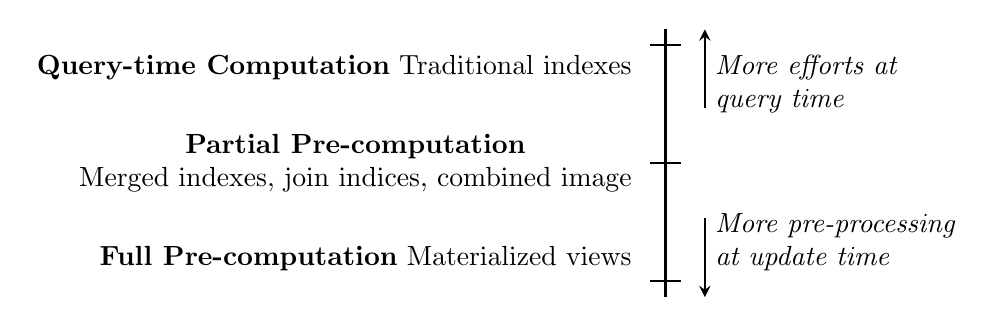
\begin{tikzpicture}[>=stealth, thick]
        \draw[-, very thick] (0,-0.2) -- (0,3.2);
        \draw[<-] (0.5,-0.2) -- (0.5,0.8);
        \node[align=left, anchor=south west, font=\itshape] at (0.5,0) {More pre-processing\\at update time};
        \draw[->] (0.5,2.2) -- (0.5,3.2);
        \node[align=left, anchor=north west, font=\itshape] at (0.5,3) {More efforts at\\query time};
        
        % Bottom Node: Query-time Computation
        \draw (-0.2, 0) -- (0.2, 0);
        \node[align=center, left=0.3cm, anchor=south east] at (0,0) (query_time) {\textbf{Full Pre-computation} Materialized views};

        % Middle Node: Merged Indexes
        \draw (-0.2, 1.5) -- (0.2, 1.5);
        \node[align=center, left=0.3cm] at (0,1.5) (partial_precomp) {\textbf{Partial Pre-computation}\\Merged indexes, join indices, combined image};

        % Top Node: Full Pre-computation
        \draw (-0.2, 3) -- (0.2, 3);
        \node[align=center, left=0.3cm, anchor=north east] at (0,3) (full_precomp) {\textbf{Query-time Computation} Traditional indexes};
        
    \end{tikzpicture}
    }
    \Description{A vertical line representing a spectrum. At the bottom is `Query-time Computation' with `Traditional indexes' below it. In the middle is `Partial Pre-computation' with `Merged indexes, join indices, combined image' to the right. At the top is `Full Pre-computation' with `Materialized views' to the left. An arrow points down, labeled `More efforts at query time'. An arrow points up, labeled `More pre-processing at update time'.}
    \caption{Spectrum of Pre-computation.\textnormal{
    The vertical axis represents the continuum of workload distribution: query-time work increases downward, and update-time pre-processing increases upward.
    Merged indexes occupy the middle ground, i.e., ``partial pre-computation''.
}}\label{fig:spectrum_precomputation}
\end{figure}

Relational database systems typically compute a query on the fly (i.e., at query time). 
They may run moderate pre-processing on database updates to later accelerate query execution, typically in the form of index creation and index maintenance.
Columnar stores often perform even less pre-processing at update time since they may not maintain ordered indexes.
This represents one extreme that devotes almost all effort to query time.

On the other end, materialized views fully pre-compute and store a query, shifting almost all effort to update time. 
At query time, databases only perform a simple retrieval from a materialized view (often an index retrieval from an indexed view~\cite{indexedviews}).
They pay the cost of view storage and view maintenance at update time.
Some database systems refresh materialized join views only occasionally, and each refresh requires a full re-evaluation of the query~\cite{ibm2024mqts, postgresql2024incremental}.
Incremental view maintenance (IVM) greatly mitigates this cost~\cite{gupta1995maintenance,Zhuge1995ViewMaintenance,Blakeley1990PerformanceAnalysis,GUPTAchangetable,mumick1997maintenance,larson2007outerjoin}.
However, many systems impose strict constraints on which views can be incrementally maintained, such as lack of support for outer joins~\cite{mysql2024viewupdatability,indexedviews,databricks2018stream}.
Oracle's support for IVM is impressively comprehensive, despite the complexity and remaining constraints~\cite{oracle2024mvrefresh}.

\begin{sloppypar}
Recent academic studies have proposed several high-performance IVM engines, but they also present some trade-offs.
DBToaster~\cite{dbtoaster, f-ivm, dbtoasterFK} and Naiad~\cite{mcsherry2013differentialdataflow,budiu2025dbsp} achieve excellent IVM performance by maintaining intermediate views and differential traces in memory, respectively.
However, their memory consumption, especially that of the former, can be prohibitive for large datasets.
Umbra~DB's ``split maintenance''~\cite{umbra20} achieves both a high insert rate and low query latency, but it lacks support for joins without a subsequent aggregation.
\end{sloppypar}

\subsection{Partial Pre-computation}\label{subsec:partial-precomp}

The middle ground of the pre-computation spectrum, as shown in Figure~\ref{fig:spectrum_precomputation}, is partial pre-computation. Some studies propose storage structures that require less pre-processing than materialized views but more than traditional indexes.

\begin{sloppypar}
Two classic studies, join indices~\cite{oneil1995joinindex,valduriez87joinindex} and combined images~\cite{haerder1978combined}, are the conceptual predecessors of merged indexes.
As Table~\ref{tab:partial-precomp} lays out, join indices store base row IDs (e.g., \( (r_\text{id}, s_\text{id}, t_\text{id}) \)) of each joined row.
Combined images co-group the rows without joining them, mapping each join key to sets of matching row IDs in each relation.
In comparison, merged indexes generalize combined images by storing actual records (or selected columns) per key.
\end{sloppypar}

\begin{table}[htbp]
    \small
    \centering
        \caption{Join index~\cite{oneil1995joinindex,valduriez87joinindex}, combined image~\cite{haerder1978combined}, and merged index. \textnormal{This table summarizes these storage structures for computation of \(R \bowtie S \bowtie T\). \(r_\text{id}\) represents the row ID of a record in relation \(R\), and \(\pi(r)\) represents the projection of a record \(r\).}}\label{tab:partial-precomp}
    \begin{tabular}{r l l}
        \toprule
        & Content & Cardinality \\
        \midrule
        Join& \( (r_\text{id}, s_\text{id}, t_\text{id}) \) & \( |R \bowtie S \bowtie T| \)\\
        index & Joined row IDs & \\
        \cmidrule{1-3}
        Combined&key \(\rightarrow (\{r_\text{id}\}, \{s_\text{id}\}, \{t_\text{id}\})\)&Count of unique keys,\\
        image & Co-grouped row IDs  & which is no more than\\
        && \( |R| + |S| + |T| \)\\
        \cmidrule{1-3}
        Merged&key \(\rightarrow\)& \( |R| + |S| + |T| \)\\
        index &\((\{\pi(r)\}, \{\pi(s)\}, \{\pi(t)\})\)&\\
        & Co-grouped records & \\
        & or their projection & \\
        \bottomrule
    \end{tabular}
\end{table}

Recent techniques for partial pre-computation---often introduced under the broad umbrella of IVM, since they represent alternatives to traditional materialized views---appear in the following studies.
\footnote{
Some IVM techniques reviewed in Section~\ref{subsec:precomputation_vs_querytime} use auxiliary data structures to accelerate view maintenance.
These auxiliary structures are not classified as partial pre-computation because their ultimate target remains a fully pre-computed materialized view, and they cannot answer queries independently.
In comparison, the partial pre-computation techniques reviewed here can answer queries like materialized views do, though they require a variable degree of query-time computation and participation of base tables.
}
Factorized IVM~\cite{f-ivm, factorizedDB} stores factorized representations of query results, but it only offers an in-memory implementation.
\Citet{Berkholz2017conjunctive,Idris2017DyanmicYanakakis} offer strong theoretical guarantees but target main-memory environments. 
IQP~\cite{iqp} persists and maintains intermediate states of query processing, most notably hash tables. 
Symmetric hash tables~\cite{wilschut1991shj, hong1993shj, Urhan2000XJoinAR, lawrence2005early} may also be considered a form of partial pre-computation.
These hash-based approaches are highly complementary to our work's focus on order-based query operators.

\subsection{Merged Index and its Advantage in Two-table Joins}\label{subsec:two_table_merged}

Our two previous studies proposed merged indexes~\cite{graefe2007merged} and showed their advantage for two-table joins~\cite{lyu2025indexing}.
Merged indexes belong to a broader lineage of multi-table clustering strategies.
Object-oriented database systems~\cite{DARMONT199655} are the earliest example; by contrast, merged indexes, thanks to physical data independence, implement clustering while upholding the relational model.
More recently, the idea of clustering has surfaced in diverse contexts, including distributed systems (e.g., Google Flume's ``co-group-by''~\cite{beam2024cogroupbykey} and Spanner's interleaved tables~\cite{spanner13}), NoSQL systems (e.g., Cassandra's wide partition~\cite{carpenter2022cassandra}), and even columnar storage (e.g., nested data~\cite{dremel,Rey2023nested}).

\subsubsection{Design of merged indexes~\cite{graefe2007merged}}
A merged index~\cite{graefe2007merged} maps a search key to a set of records from different tables, as summarized in Table~\ref{tab:partial-precomp}. The mapping is accomplished by a sort order that physically interleaves records from multiple tables and clusters records sharing a common key.
The interleaving and clustering within a merged index rely on a record structure that accommodates variable record types and key structures. As shown in Figure~\ref{fig:record_structure}, the physical format of a record consists of three components:

\textbf{Key structure with domain tags:} The domain tag before each key field acts as a separator and a domain identifier (domains are types of key columns). This enables byte-wise comparison of composite keys that may differ in depth.\footnote{The design of domain tags not only allows variable-length keys without inefficient NULL paddings but also allows keys of the same length to be differentiated, such as \texttt{(N:`USA';S:`WI';GOV:`Tony Evers')} versus \texttt{(N:`USA';S:`WI';CO:`Dane')}.} Therefore, any storage format must accommodate variable-length keys if they underlie the implementation of merged indexes.

\textbf{Index identifier:} Immediately following the key, a special domain tag (\texttt{I} in Figure~\ref{fig:record_structure}) indicates the end of the key and the start of the index identifier. An index identifier identifies the source index of the record. Index identifiers can also be part of the sort key, enabling the interleaving of records with the same join key but different source indexes.\footnote{Merged indexes allow two entries with exactly the same key and index identifier, but specific storage implementation may not, such as LeanStore~\cite{leanstore18}. However, this limitation can be sidestepped by appending the primary key of the source table after the index identifier as part of the sort key.}

\textbf{Payload:} The remaining non-key columns of a record are stored as the payload following the index identifier, usually in a binary format without any special tags and requiring parsing based on schema information. It does not participate in the sort order.

\begin{figure}[htbp]
    \centering
    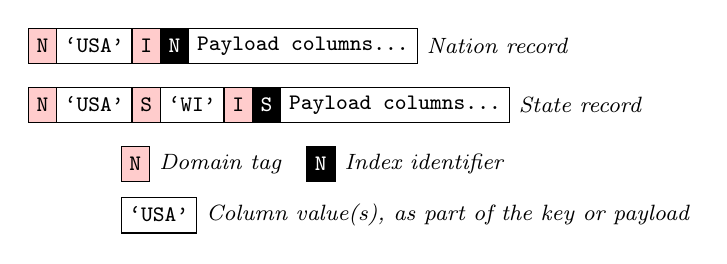
\begin{tikzpicture}[
        % Define a standard style for all boxes to keep code clean
        box/.style={draw, inner sep=3pt,
        font=\ttfamily\footnotesize,
        minimum height=0.45cm, outer sep=0pt},
        % Style for the label text outside boxes
        labeltext/.style={font=\footnotesize\itshape, anchor=west}
    ]

    % --- Row 1: Nation Record ---
    % 1. Nation Tag
    \node[box, fill=red!20] (nrec_ntag) {N};
    
    % 2. Nation Key (placed relative to the tag)
    \node[box, anchor=west] (nrec_nkey) at (nrec_ntag.east) {`USA'};
     
    % 3. Index ID
    \node[box, fill=red!20, anchor=west] (nrec_itag) at (nrec_nkey.east) {I};
    \node[box, fill=black, text=white, anchor=west] (nrec_idx) at (nrec_itag.east) {N};
    
    % 4. Payload
    \node[box, anchor=west] (nrec_payload) at (nrec_idx.east) {Payload columns...};
    \node[labeltext] (nrec_legend) at (nrec_payload.east) {Nation record};
    
    % --- Row 2: State Record ---
    % We place the first node of this row below the first node of the previous row
    \node[box, fill=red!20, anchor=north west, yshift=-0.3cm] (srec_ntag) at (nrec_ntag.south west) {N};
    
    % 2. Nation Key (Common Prefix)
    \node[box, anchor=west] (srec_nkey) at (srec_ntag.east) {`USA'};
    
    % 3. State Tag
    \node[box, fill=red!20, anchor=west] (srec_stag) at (srec_nkey.east) {S};
    
    % 4. State Key
    \node[box, anchor=west] (srec_skey) at (srec_stag.east) {`WI'};
    
    % 5. Index ID
    \node[box, fill=red!20, anchor=west] (srec_itag) at (srec_skey.east) {I};
    \node[box, fill=black, text=white, anchor=west] (srec_idx) at (srec_itag.east)  {S};
    
    % 6. Payload
    \node[box, anchor=west] (srec_payload) at (srec_idx.east) {Payload columns...};
    \node[labeltext] (srec_legend) at (srec_payload.east) {State record};
    
    % --- Legend ---
    % Placed below the second row
    \node[box, fill=red!20, anchor=north west, yshift=-0.3cm, xshift=1cm] (ntag) at (srec_ntag.south) {N};
    \node[labeltext] (ntag_legend) at (ntag.east) {Domain tag};
    
    \node[box, fill=black, text=white, anchor=west, xshift=0.2cm] (idx) at (ntag_legend.east) {N};
    \node[labeltext] (idx_legend) at (idx.east) {Index identifier};
    
    \node[box, anchor=north west, yshift=-0.2cm] (nkey) at (ntag.south west) {`USA'};
    \node[labeltext] (nkey_legend) at (nkey.east) {Column value(s), as part of the key or payload};

    \end{tikzpicture}
    \caption{Record structure in a merged index with variable-length keys. \textnormal{
    Each record consists of a sort key with domain tags, an index identifier led by a domain tag, and a payload.
    Adapted from Figure 3 by \citet{graefe2007merged}.
    }}\label{fig:record_structure}
    \Description{A diagram showing the structure of two records in a merged index. The first record, a Nation record, consists of a domain tag `N', a key value `USA', an index identifier `N', and a payload. The second record, a State record, shows a hierarchical key structure. It has a domain tag `N', a key value `USA', another domain tag `S', a key value `WI', an index identifier `S', and a payload. A legend at the bottom explains that colored boxes are domain tags, black boxes are index identifiers, and white boxes are column values.}
\end{figure}

\subsubsection{Merged indexes for two-table joins}
\citet{lyu2025indexing} recommended merged indexes for two-table joins, because they excel simultaneously in query performance, update performance, and space efficiency.
A merged index is a hybrid between the equivalent traditional indexes and the equivalent two-table join view. On one hand, a two-table merged index is simply a reorganization (interleaving by sort order) of the two single-table indexes. On the other hand, by co-locating matching entries from two indexes, the merged index partially pre-computes the join and is only one step away (i.e., the step of record assembly) from the materialized view.

\summary{Summary of related work and research goal of this work}\label{para:research_goal} 
On the foundation of prior work reviewed above, this study aims to generalize merged indexes to multi-table queries described by interesting orderings.
Traditional approaches to these query pipelines present trade-offs among query performance, update performance, and space efficiency.
Partial pre-computation techniques, the middle ground between traditional approaches, have seen recent interest but impose trade-offs or limitations.
This study proposes a technique of partial pre-computation and investigates whether and how, similar to two-table merged indexes, multi-table merged indexes can break the classic trade-off.

% --- Technique Section ---
\section{Structure of Multi-table Merged Indexes---``Data at Rest''}\label{sec:structure_at_rest} 

A merged index organizes multiple types of records according to a shared sort order and can store and index inputs for two-table joins. This section generalizes this structure to support multi-table joins and groupings on shared keys.
Sections~\ref{subsec:int_ord_cluster} and~\ref{subsec:int_ord_group} discuss how multi-table merged indexes embed interesting orderings for multi-table joins and multi-table aggregations, respectively. Section~\ref{subsec:storage_spectrum} compares multi-table merged indexes with row-oriented and columnar storage.
Section~\ref{sec:space_implementation} discusses storing views in merged indexes, as well as the space requirements and the implementation of multi-table merged indexes.

\subsection{Embedding Interesting Orderings for Multi-table Joins}\label{subsec:int_ord_cluster}

Multi-table joins that share a sort order can either have identical join keys or join keys that form a prefix chain.
Merged indexes can embed both types of interesting orderings, as discussed in Sections~\ref{sssec:identical_join_keys} and~\ref{sssec:hierarchical_join_keys}, respectively.

Multi-table joins with shared keys often arise from the reconstruction of complex application objects from multiple normalized tables. As Section~\ref{subsec:normal_forms} points out, frequent join patterns like these and database schema design (using the idea of complex application objects) often coincide.
This section shows how both factors drive the physical design of merged indexes.

\subsubsection{Sort order for multi-table joins with identical join keys}\label{sssec:identical_join_keys}

For multi-table joins where the join keys are exactly the same, a merged index sorts all records by the join key and creates the simplest shared sort order defined by a single column set.

Consider Query~\ref{lst:cust_join} for an example. From the perspective of complex application objects, it reconstructs the complex application object as shown in Figure~\ref{fig:er-cust}---a customer with all their orders and invoices. 
The traditional optimization technique of interesting orderings may generate a plan as shown in Figure~\ref{fig:cust_join_int_order} for Query~\ref{lst:cust_join}---since the joined result of Customer and Orders is already sorted on \texttt{custkey}, the second merge join can directly consume the intermediate result without a sort phase.

\begin{queryblock}
\begin{lstlisting}[
    caption={Three-way join of Customer, Orders, and Invoice on \texttt{custkey}.}, 
    label={lst:cust_join}
]
SELECT * FROM Customer 
    JOIN Orders ON Customer.custkey = Orders.custkey
    JOIN Invoice ON Orders.custkey = Invoice.custkey;
\end{lstlisting}
\Description{A SQL query joining three tables (Customer, Orders, and Invoice) on a common key.}
\end{queryblock}

\begin{figure}[htbp]
    \centering

    \begin{subfigure}[t]{0.48\linewidth}
        \centering
        \resizebox{\linewidth}{!}{%
        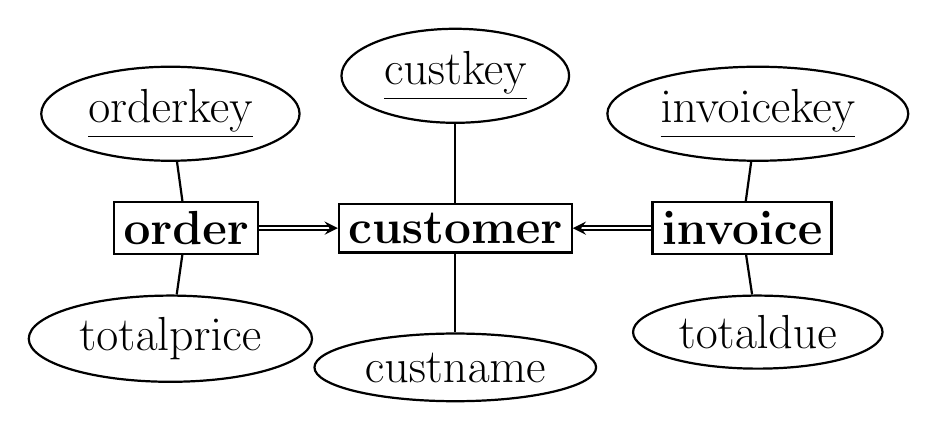
\begin{tikzpicture}[
            >=stealth, thick,
            attr/.style={draw, ellipse, thick, minimum width=4mm, minimum height=2mm, font=\LARGE},
            entity/.style={draw, rectangle, thick, minimum size=5mm, font=\bfseries\LARGE}
        ]
            % Customer
            \node[entity] (cust) {customer};
            \node[attr, anchor=south, above=1 of cust] (custkey) {\underline{custkey}};
            \node[attr, anchor=north, below=1 of cust] (custname) {custname};
            \draw (cust) -- (custkey);
            \draw (cust) -- (custname);
            
            % Orders
            \node[entity, anchor=east, left=of cust] (order) {order};
            \node[attr, anchor=south, above=0.5 of order, xshift=-2mm] (orderkey) {\underline{orderkey}};
            \node[attr, anchor=north, below=0.5 of order, xshift=-2mm] (totalprice) {totalprice};
            \draw (order) -- (orderkey);
            \draw (order) -- (totalprice);

            % Invoice
            \node[entity, anchor=west, right=of cust] (invoice) {invoice};
            \node[attr, anchor=south, above=0.5 of invoice, xshift=2mm] (invoicekey) {\underline{invoicekey}};
            \node[attr, anchor=north, below=0.5 of invoice, xshift=2mm] (totaldue) {totaldue};
            \draw (invoice) -- (invoicekey);
            \draw (invoice) -- (totaldue);

            \draw[double, <-] (cust) -- (order);
            \draw[double, ->] (invoice) -- (cust);
        \end{tikzpicture}%
        }
        \Description{Entity-relationship diagram of a customer with orders and invoices; underlined keys, arrows denote many-to-one, double lines total participation.}
        \subcaption{ER diagram showing a customer as a complex application object with orders and invoices.}\label{fig:er-cust}
    \end{subfigure}
    \hfill
    \begin{subfigure}[t]{0.48\linewidth}
        \centering
        \resizebox{\linewidth}{!}{%
        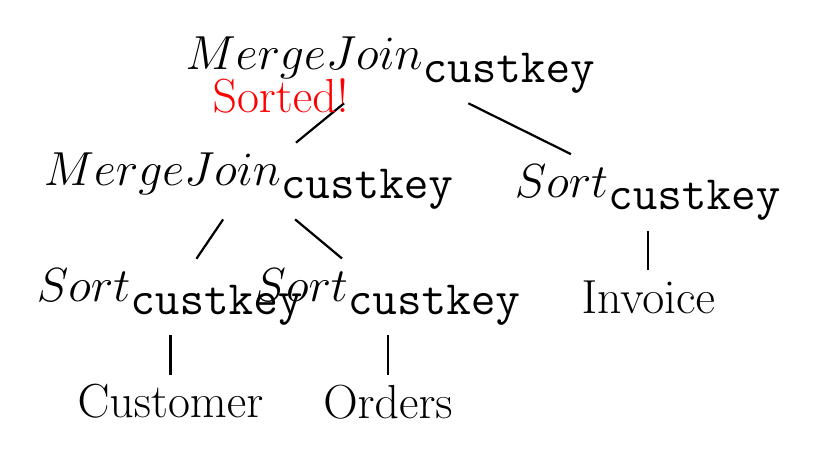
\begin{tikzpicture}[thick, font=\LARGE]
            \node (scan_cust) {Customer};
            \node[anchor=south, above=0.5 of scan_cust] (sort_cust) {$\text{Sort}_{\texttt{custkey}}$};
            \draw (scan_cust) -- (sort_cust);
            \node[anchor=south, above=0.5 of sort_cust, xshift=10mm, font=\LARGE] (merge_cust_order) {$\text{Merge Join}_{\texttt{custkey}}$};
            \draw (sort_cust) -- (merge_cust_order);

            \node[anchor=west, right=0.5 of scan_cust] (scan_order) {Orders};
            \node[anchor=south, above=0.5 of scan_order] (sort_order) {$\text{Sort}_{\texttt{custkey}}$};
            \draw (sort_order) -- (scan_order);
            \draw (sort_order) -- (merge_cust_order);

            \node[anchor=south, above=0.5 of merge_cust_order, xshift=18mm, font=\LARGE] (merge_cust_order_invoice) {$\text{Merge Join}_{\texttt{custkey}}$};
            \draw (merge_cust_order) -- (merge_cust_order_invoice);
            \node[anchor=south east, above=0.25 of merge_cust_order, xshift=4mm, color=red] (sorted) {Sorted!};
            
            \node[anchor=west, right=0.5 of sort_order] (scan_invoice) {Invoice};
            \node[anchor=south, above=0.5 of scan_invoice] (sort_invoice) {$\text{Sort}_{\texttt{custkey}}$};
            \draw (scan_invoice) -- (sort_invoice);
            \draw (sort_invoice) -- (merge_cust_order_invoice);
        \end{tikzpicture}%
        }
        \Description{Query plan with sorts on custkey and consecutive merge joins exploiting interesting orderings.}
        \subcaption{A traditional query optimizer may generate a plan with interesting orderings.}\label{fig:cust_join_int_order}
    \end{subfigure}
    \caption{Schema and query plan for Query~\ref{lst:cust_join}.}\label{fig:cust_join}

\end{figure}

In comparison to this traditional plan that recognizes interesting orderings at the time of \textit{query planning}, a merged index embeds this shared sort order into \textit{the physical design}.
For this query, a merged index should store the primary index of the Customer table and the secondary indexes keyed on \texttt{custkey} of the Orders and Invoice tables.
Thus, merged indexes embed the shared sort order of multiple types of records required by the joins.
This synergy between query optimization and physical design is seen in established practices---using indexes as pre-sorted inputs for merge joins to eliminate explicit sorting during query execution.

In our design, merged indexes, by default, store all columns required by the queries, enabling index-only retrieval and eliminating the need to access base tables during query execution.
This merged index effectively creates ``master-detail clustering''~\cite{graefe2007merged} for this customer object. The shared sort order physically co-locates master records (e.g., customer records) and detail records (e.g., order records and invoice records) from distinct logical tables. 
By exploiting physical data independence, this design achieves clustering for complex application objects while maintaining the integrity of the normalized relational schema.

\subsubsection{Hierarchical sort order for multi-table joins with ``hierarchical join keys''}\label{sssec:hierarchical_join_keys}

Merged indexes also support queries where the join keys are ``hierarchical subsets'', as these keys define compatible sort orders. 
Sort orders are compatible when the keys form a prefix chain, since lexicographical sorting by a composite key (e.g., \texttt{(A, B)}) preserves the order of its prefix (e.g., \texttt{A}).
A single shared order on the maximal key satisfies the merge join requirements on all subset keys. This is possible because the record structure of merged indexes allows composite keys.
% LTeX: enabled=false
Query~\ref{lst:geo_join} is an example of multi-table joins with hierarchical join keys. In the chain of joins, the join keys extend from \texttt{(nationkey)} to \texttt{(nationkey, statekey, countykey)}. Query optimization by interesting orderings may generate a plan of three consecutive merge joins, sorting only the inputs and exploiting the sorted nature of intermediate joined results.
In comparison, a merged index should store the primary indexes of the four tables, sorted by \texttt{(nationkey, statekey, countykey, citykey)}. Figure~\ref{fig:interleaved_storage} illustrates such a merged index stored in the B-tree format.
Sorting multiple types of records requires a special format of keys.
As shown in Figure~\ref{fig:records_interleaved}, each record includes key columns with domain tags (e.g., \texttt{N05 S02 C01 IC})\footnote{
    These tags are technically 3-bit values, required to distinguish the four domain types and the index identifier, but for readability, they are represented here as \texttt{N}, \texttt{S}, \texttt{C}, and \texttt{T} for Nation, States, County, and City. \texttt{I} is the domain tag for the index identifier. Similar illustrations also apply to index identifiers.
    }, index identifiers (e.g., \texttt{IT}), and payload columns.
See Figure~\ref{fig:record_structure} in Section~\ref{subsec:two_table_merged} for details of the record structure in merged indexes.
% LTeX: enabled=true

\begin{queryblock}
\begin{lstlisting}[
    caption={Four-way join of Nation, States, County, and City on hierarchical join keys.}, 
    label={lst:geo_join}
]
SELECT *
FROM Nation AS n JOIN States AS s ON n.nationkey = s.nationkey
JOIN County AS c
    ON s.nationkey = c.nationkey AND s.statekey = c.statekey
JOIN City AS ci
    ON c.nationkey = ci.nationkey AND c.statekey = ci.statekey AND c.countykey = ci.countykey;
\end{lstlisting}
\Description{A SQL query joining four tables (Nation, States, County, and City) on hierarchical keys.}
\end{queryblock}
\begin{figure}[htbp]
    \centering
    \begin{subfigure}{\linewidth}
    \resizebox{\linewidth}{!}{
    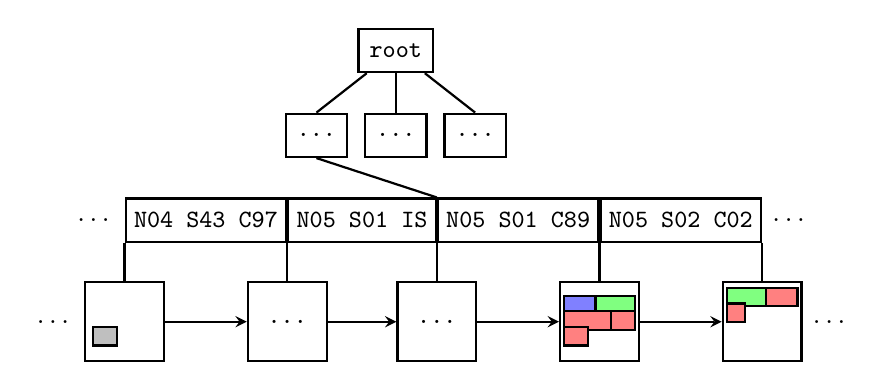
\begin{tikzpicture}[
        % Standard style for the record rows
        thick, >=stealth,
        btreenode/.style={
            draw,
            rectangle,
            minimum width=0.55cm,
            minimum height=0.55cm,
            font=\ttfamily\small,
            align=left,
            anchor=north,
            inner sep=4pt
        },
        bkey/.style={
            draw,
            minimum height=0.55cm,
            font=\ttfamily\small,
            align=center,
            inner sep=3pt
        },
        btreeleaf/.style={
            draw,
            rectangle,
            minimum width=1cm,
            minimum height=1cm,
            font=\ttfamily\small,
        },
        leafrecord/.style={
            draw, rectangle, minimum height=0.1cm, anchor=west
        },
        nationrec/.style={leafrecord, fill=gray!50},
        staterec/.style={leafrecord, fill=blue!50},
        countyrec/.style={leafrecord, fill=green!50},
        cityrec/.style={leafrecord, fill=red!50}
        ]

        \node [btreenode] (root) {root};
        \node [btreenode, yshift=-0.5cm] (branch_j2) at (root.south) {\dots};
        \draw (root) -- (branch_j2.north);
        \node [btreenode, xshift=-0.2cm, anchor=east] (branch_j1) at (branch_j2.west) {\dots};
        \draw (root) -- (branch_j1.north);
        
        \node [btreenode, anchor=west, xshift=0.2cm] (branch_j3) at (branch_j2.east) {\dots};
        \draw (root) -- (branch_j3.north);

        \node [bkey, yshift=-0.5cm, xshift=-1cm, anchor=north] (branch_k1) at (branch_j1.south west) {N04 S43 C97};
        \node [bkey, anchor=west] (branch_k2) at (branch_k1.east) {N05 S01 IS};
        \node [bkey, anchor=west] (branch_k3) at (branch_k2.east) {N05 S01 C89};
        \node [bkey, anchor=west] (branch_k4) at (branch_k3.east) {N05 S02 C02};
        \draw (branch_j1.south) -- (branch_k2.north east);


        \node [anchor=east] (dots2-1) at (branch_k1.west) {\dots};
        \node [anchor=west] (dots2-2) at (branch_k4.east) {\dots};
        
        \node [btreeleaf, yshift=-1cm] (leaf1) at (branch_k1.south west) {};
        \draw (branch_k1.south west) -- (leaf1.north);
        \node[anchor=east] (leafdots1) at (leaf1.west) {\dots};
        \node [nationrec, minimum width=0.3cm, xshift=0.1cm, yshift=-0.7cm] (n05) at (leaf1.north west) {};

        \node [btreeleaf, yshift=-1cm] (leafdots1) at (branch_k1.south east) {\dots};
        \draw (branch_k1.south east) -- (leafdots1.north);

        \node [btreeleaf, yshift=-1cm] (leafdots2) at (branch_k2.south east) {\dots};
        \draw (branch_k2.south east) -- (leafdots2.north);

        \node [btreeleaf, yshift=-1cm] (leaf2) at (branch_k3.south east) {};
        \draw (branch_k3.south east) -- (leaf2.north);
        \node [staterec, minimum width=0.4cm, xshift=0.05cm, yshift=-0.3cm] (s32) at (leaf2.north west) {};
        \node [countyrec, minimum width=0.5cm, xshift=0.45cm, yshift=-0.3cm] (c01) at (leaf2.north west) {};
        \node [cityrec, minimum width=0.6cm, xshift=0.05cm, yshift=-0.5cm] (T01) at (leaf2.north west) {};
        \node [cityrec, minimum width=0.3cm, xshift=0.65cm, yshift=-0.5cm] (T01cont) at (leaf2.north west) {};
        \node [cityrec, minimum width=0.3cm, xshift=0.05cm, yshift=-0.7cm] (T02) at (leaf2.north west) {};
        
        \node [btreeleaf, yshift=-1cm] (leaf3) at (branch_k4.south east) {};
        \draw (branch_k4.south east) -- (leaf3.north);
        \node [countyrec, minimum width=0.5cm, xshift=0.05cm, yshift=-0.2cm] (c02) at (leaf3.north west) {};
        \node [cityrec, minimum width=0.4cm, xshift=0.55cm, yshift=-0.2cm] (T03) at (leaf3.north west) {};
        \node [cityrec, minimum width=0.2cm, xshift=0.05cm, yshift=-0.4cm] (T03cont) at (leaf3.north west) {};
        \node[anchor=west] (leafdots3) at (leaf3.east) {\dots};

        \draw[->] (leaf1) -- (leafdots1);
        \draw[->] (leafdots1) -- (leafdots2);
        \draw[->] (leafdots2) -- (leaf2);
        \draw[->] (leaf2) -- (leaf3);
        \end{tikzpicture}
    }
    \subcaption{Merged index as stored in a B-tree. The branch nodes sort multiple types of records by a hierarchical key. The leaf nodes interleave and cluster records from different tables; selected records are shown with different colors.}\label{fig:btree_interleaved}
    \end{subfigure}
    \begin{subfigure}{\linewidth}
        \centering
    \begin{tikzpicture}[
        field/.style={
            draw,
            rectangle,
            minimum height=0.55cm,
            minimum width=0.8cm,
            font=\ttfamily\footnotesize,
            align=center,
            anchor=north west,  
            inner sep=0pt
        },
        prefix_style/.style={
            draw=gray!50,
            text=gray!50,
            fill=none
        },
        idxid/.style={
            draw,
            rectangle,
            minimum height=0.55cm,
            minimum width=0.6cm,
            align=center,
            inner sep=0pt,
            font=\ttfamily\footnotesize,
            anchor=north west
        },
        recordcont/.style={
            draw,
            rectangle,
            minimum height=0.55cm,
            minimum width=1.4cm,
            align=left,
            inner sep=4pt,
            font=\sffamily\footnotesize,
            anchor=north west
        }
    ]
    
    % Row 1: Nation
    \node[field, fill=gray!10, yshift=-1cm] (r1-n) at (leaf1.south west) {N05};
    \node [idxid, fill=gray!10] (r1-1) at (r1-n.north east) {IN};
    \node [recordcont, fill=gray!10] (r1-2) at (r1-1.north east) {`USA'};
    % \draw[gray, ->] (n05.south) -- (r1-2.north);

    % Row 2: State (Child of USA)
    \node[field, prefix_style] (r2-n) at (r1-n.south west) {N05};
    \node[field, fill=blue!10] (r2-s) at (r2-n.north east) {S02};
    \node [idxid, fill=blue!10] (r2-1) at (r2-s.north east) {IS};
    \node [recordcont, fill=blue!10] (r2-2) at (r2-1.north east) {`WI'};
    % \draw [blue, ->] (s32.south) -- (r2-2.north);

    % Row 3: County (Child of WI)
    \node[field, prefix_style] (r3-n) at (r2-n.south west) {N05};
    \node[field, prefix_style] (r3-s) at (r3-n.north east) {S02};
    \node[field, fill=green!10] (r3-c) at (r3-s.north east) {C01};
    \node [idxid, fill=green!10] (r3-1) at (r3-c.north east) {IC};
    \node [recordcont, fill=green!10] (r3-2) at (r3-1.north east) {`Dane'};
    % \draw [green, ->] (c01.south) -- (r3-2.north);

    % Row 4: City (Child of Dane)
    \node[field, prefix_style] (r4-n) at (r3-n.south west) {N05};
    \node[field, prefix_style] (r4-s) at (r4-n.north east) {S02};
    \node[field, prefix_style] (r4-c) at (r4-s.north east) {C01};
    \node[field, fill=red!10] (r4-d) at (r4-c.north east) {T01};
    \node [idxid, fill=red!10] (r4-1) at (r4-d.north east) {IT};
    \node [recordcont, fill=red!10] (r4-2) at (r4-1.north east) {`Madison'};
    % \draw [red, ->] (T01.south) -- (r4-2.north);

    % Row 5: City (Sibling of Madison)
    \node[field, prefix_style] (r5-n) at (r4-n.south west) {N05};
    \node[field, prefix_style] (r5-s) at (r5-n.north east) {S02};
    \node[field, prefix_style] (r5-c) at (r5-s.north east) {C01};
    \node[field, fill=red!10] (r5-d) at (r5-c.north east) {T02};
    \node [idxid, fill=red!10] (r5-1) at (r5-d.north east) {IT};
    \node [recordcont, fill=red!10] (r5-2) at (r5-1.north east) {`Fitchburg'};
    % \draw [red, ->] (T02.south) -- (r5-2.north);

    % Row 6: County (Sibling of Dane)
    \node[field, prefix_style] (r6-n) at (r5-n.south west) {N05};
    \node[field, prefix_style] (r6-s) at (r6-n.north east) {S02};
    \node[field, fill=green!10] (r6-c) at (r6-s.north east) {C02};
    \node [idxid, fill=green!10] (r6-1) at (r6-c.north east) {IC};
    \node [recordcont, fill=green!10] (r6-2) at (r6-1.north east) {`Sauk'};
    % \draw [green, ->] (c02.south) -- (r6-2.north);

    % Row 7: City (Child of Sauk)
    \node[field, prefix_style] (r7-n) at (r6-n.south west) {N05};
    \node[field, prefix_style] (r7-s) at (r7-n.north east) {S02};
    \node[field, prefix_style] (r7-c) at (r7-s.north east) {C02};
    \node[field, fill=red!10] (r7-d) at (r7-c.north east) {T01};
    \node [idxid, fill=red!10] (r7-1) at (r7-d.north east) {IT};
    \node [recordcont, fill=red!10] (r7-2) at (r7-1.north east) {`Baraboo'};
    % \draw [red, ->] (T03.south) -- (r7-2.north);
    \end{tikzpicture}
    \subcaption{Example records from the merged index, corresponding to the colored blocks in Figure~\ref{fig:btree_interleaved}.
        Parent prefixes are shown in gray, creating vertical indentations that represent the depths of the hierarchy: Nation \(\to\) State \(\to\) County \(\to\) City.}\label{fig:records_interleaved}
    \end{subfigure}
        \caption{The layout of a multi-table merged index for the geographical four-table join.
    }\label{fig:interleaved_storage}
    \Description{A two-part figure illustrating a multi-table merged index. Part (a) shows a B-tree structure where leaf nodes contain interleaved records from four tables (Nation, State, County, City), represented by colored blocks. Part (b) gathers these records and shows hierarchical keys creating an indented and nested layout that reflects the relationships between tables.}
\end{figure}


Compared with a traditional B-tree index, the branch nodes in Figure~\ref{fig:btree_interleaved} store keys of variable lengths up to the index identifiers in order to sort and interleave all types of records.
The leaf nodes store the actual records, with different colors representing different record types.
Figure~\ref{fig:records_interleaved} shows example records from this merged index, corresponding to the colored blocks in the leaf nodes.
The three cities and their parent records form three city objects.
All records but one reside in two adjacent leaf nodes.
Since the entire nation object is very large, spanning multiple pages, some child records are separated from the ancestor record by the large amount of siblings.
This phenomenon may affect the performance of merged indexes, but the experiments do not show significant degradation, as Section~\ref{sec:experiments} will discuss.

\summary{Summary of Section~\ref{subsec:int_ord_cluster}}\label{para:rest_notes}

The physical layout of merged indexes materializes interesting orderings for multi-table joins with both identical join keys and those that form a hierarchical prefix chain. As this structure clusters matching records required by the joins, these clusters often represent instances of a complex application object.

\subsection{Embedding Interesting Orderings for Multi-table Aggregations}\label{subsec:int_ord_group}

Merged indexes also support queries with joins and grouping operators, all sharing a sort order. They permit various placements of grouping operators in the query plan (e.g., before or after joins). From the perspective of complex application objects, such queries often arise from the need to compute aggregate statistics over collections of related items within object instances, namely, complex-object summaries.
Both the query patterns and the schema design drive the physical design of merged indexes, similar to the case of multi-table joins discussed in Section~\ref{subsec:int_ord_cluster}.

Query~\ref{lst:geo_mixed} is an example of grouping operators placed after the joins.
Similar to multi-table joins, the join keys and grouping keys can be identical column sets or form a prefix chain, and Query~\ref{lst:geo_mixed} illustrates the latter case.\footnote{An example of grouping before the joins with identical column sets as the shared key is omitted for brevity but can be found in the artifact repository at \url{\vldbavailabilityurl}.}
This query summarizes the number of cities in each state.
The sort order defined by the finest join key, \texttt{(nationkey, statekey, countykey)}, also satisfies the grouping requirement (by \texttt{(nationkey, statekey)}).

\begin{queryblock}
\begin{lstlisting}[
    caption={Mixed query joining Nation, States, County, and City on hierarchical join keys, with a final grouping operation.}, 
    label={lst:geo_mixed}
]
SELECT nationkey, n_name, statekey, s_name, COUNT(*)
FROM Nation AS n 
    JOIN States AS s ON n.nationkey = s.nationkey
    JOIN County AS c
        ON s.nationkey = c.nationkey AND s.statekey = c.statekey
    JOIN City AS ci
        ON c.nationkey = ci.nationkey AND c.statekey = ci.statekey AND c.countykey = ci.countykey
GROUP BY nationkey, n_name, statekey, s_name
\end{lstlisting}
\Description{A SQL query joining four tables (Nation, States, County, City) and grouping the results.}
\end{queryblock}


A traditional query optimizer may generate a plan with three consecutive merge joins, followed by a sort-based grouping operator on \texttt{(nationkey, statekey)}.
The output from the three merge joins is already sorted on \texttt{(nationkey, statekey)}, satisfying the grouping requirement.\footnote{The grouping key includes other columns, \texttt{n\_name, s\_name}, but because they are functionally dependent on the join keys, they do not need to participate in the actual grouping operation. Admittedly, not all database systems optimize such functional dependencies.}
In comparison, a merged index storing the primary indexes of all four tables embeds the interesting orderings into physical storage.
The finest clusters are counties, which can be further grouped as state clusters, as needed by the grouping operation.

Notably, merged indexes also support Query~\ref{lst:order_mixed} defined upon the TPC-H schema, though the shared sort order may not be immediately obvious. The grouping key is \texttt{o\_orderpriority}, different from the join key \texttt{o\_orderkey}. However, the former is \textit{functionally dependent} on the latter. A merged index storing the primary indexes of both Orders and Lineitem tables clusters line items by their order keys. One scan of the merged index computes the sum of line item quantities grouped by each order, and the database can then aggregate these sums by order priority.

\begin{queryblock}
\begin{lstlisting}[
    caption={Query aggregating order quantities by order priority.}, 
    label={lst:order_mixed}
]
SELECT o_orderpriority, SUM (l_quantity)
FROM orders JOIN lineitem ON (o_orderkey = l_orderkey)
GROUP BY o_orderpriority
\end{lstlisting}
\Description{A SQL query that aggregates order quantities by order priority.}
\end{queryblock}

In addition, merged indexes support various aggregation functions beyond \texttt{COUNT}. They even support relatively complex aggregations, such as \texttt{MEDIAN}. For example, consider computing the median invoice amount per customer. 
Consider a merged index that stores all invoices for each customer and, within each customer cluster, sorts the invoices by their amounts.
It allows efficient median computation by directly accessing the middle record(s) of each customer cluster.
This is similar to how a traditional index storing invoices sorted by \texttt{(custkey, amountdue)} also supports this query.

Previous indexing techniques, such as join indices~\cite{oneil1995joinindex, valduriez87joinindex} and combined images~\cite{haerder1978combined}, typically target joins only. This study also supports grouping operators, unifying them with joins under shared sort orders. 
As the query optimization technique of interesting orderings, i.e., utilizing the sorted nature of intermediate results, applies to both merge joins and sort-based grouping operations~\cite{selinger1979access}, merged indexes, embedding such interesting orderings into physical storage, also support both types of operators.

\summary{Summary of Section~\ref{subsec:int_ord_group}}
Merged indexes embed interesting orderings into storage, enabling efficient query execution for multi-table aggregations sharing a sort order. They allow various placements of grouping operators in the query plan and various aggregation functions.

\subsection{Merged Indexes vs. Row and Columnar Storage}\label{subsec:storage_spectrum} 

The multi-table interesting orderings within a merged index cluster records by the sort key.
These ``record clusters'' represent units of data that the system often accesses together, specifically, matching rows required by joins and groups required by grouping operators.
One such cluster often represents a complex-object instance, such as a customer with all their orders and invoices.
As row-oriented storage groups data by row, and columnar storage groups data by column, merged indexes, taking one step further from row-oriented storage, group data by ``row cluster'' or ``record cluster''.

The popular belief is that row-oriented storage excels in OLTP workloads, and columnar storage in OLAP workloads. Following this logic, merged indexes specialize in multi-table OLTP workloads, mainly point join queries and multi-table point updates. While this is true, the strengths of merged indexes are not limited to these workloads. 
As later supported by the experiments, they also accelerate queries over longer ranges of data, as seen in operational analytics and HTAP databases, because of their support for efficient multi-table joins and grouping operations.
We leave it to future work whether merged indexes can be the unified storage for HTAP databases, so that these databases can avoid the overhead of maintaining both row stores and column stores.

\subsection{Notes on Storing Views, Space Requirements, Implementation}\label{sec:space_implementation}

\paragraph{Storing views}

While this paper focuses on merged indexes storing (indexes of) tables, merged indexes can also store views, i.e., query results.
For example, consider the merged index for Query~\ref{lst:geo_mixed}.
Instead of storing the primary index of the City table, it can store an aggregate view of the number of cities per county.\footnote{This single-table aggregate can help answer Query~\ref{lst:geo_mixed} despite the aggregation happening after the joins, as a result of ``eager aggregation''~\cite{yan95aggregate,chaudhuri94aggregate}.}
Either design choice supports Query~\ref{lst:geo_mixed}.
Supporting views in merged indexes provides a wider range of design choices, and this decision depends on the workload of the system.
The full scope of storing views in merged indexes is left to future work.

\paragraph{Space requirements}

Compared with an entry in a traditional index, only the domain tags and index identifier constitute the storage overhead of an equivalent entry in a merged index. Since a domain tag or an index identifier usually takes up only one byte, the storage overhead is minimal, as supported by the experiments.

Factorized tables~\cite{factorizedDB} can also be seen as partially executed queries so as to store the join views in a space-efficient way. Our focus on sorting and interesting orderings represents a difference in approach and scope between merged indexes and factorized tables. Our approach allows a practical implementation of merged indexes on top of ordered storage, which may be a viable, scalable, and persistent representation of factorized databases.

\paragraph{Implementation}
The primary implementation requirement for merged indexes is support for a specialized record structure with variable-length keys. Beyond this, the implementation can leverage existing components of the storage backend. For instance, sorting and indexing are delegated to the underlying ordered storage engine, and other details, such as latching mechanisms, are inherited directly.
We implemented merged indexes on two common storage backends: a B-tree (LeanStore~\cite{leanstore18}) and an LSM-tree (RocksDB~\cite{rocksdb21}). The feasibility of building merged indexes on these widely used structures suggests a practical path for their integration into existing relational database systems.

\summary{Summary of Section~\ref{sec:structure_at_rest}}

Merged indexes organize data into clusters by interleaving records; these ``record clusters'' often represent instances of complex application objects. This layout materializes the interesting orderings that enable efficient joins and groupings.
These two aspects, database schema design and query patterns, often coincide and drive the physical design of merged indexes.
Merged indexes represent a storage layout different from traditional row-oriented storage and columnar storage. Furthermore, merged indexes are space-efficient and practical to implement.
This structure lays the foundation for the high-performance query execution techniques discussed in the next section.

\section{Query Execution and Index Maintenance---``Data in Flight''}\label{sec:execution_flight}

On the foundation of the physical database design, Section~\ref{subsec:query_execution_scan} discusses query execution using merged indexes for multi-table query pipelines where the joins and grouping operations share a sort order.
Section~\ref{subsec:complex_queries} discusses the execution of complex queries where such a pipeline is only part of the entire query.
Section~\ref{subsec:maintenance} discusses the maintenance of merged indexes under data updates.
Section~\ref{subsec:spec-precomp} shows that merged indexes are a form of partial pre-computation.

\subsection{Query Execution via a Single-pass Scan}\label{subsec:query_execution_scan} 

Multi-table joins or multi-table aggregations sharing a sort order can be executed efficiently via a single-pass scan over an appropriate merged index.
Sections~\ref{sssec:multi_table_join_operator} and~\ref{sssec:multi_table_aggregation_operator} present the execution algorithm for multi-table joins and multi-table aggregations, respectively.
We presume a cost-based query optimizer that can select appropriate merged indexes and instantiate these plans when applicable.
Importantly, merged indexes are an addition to relational database systems and represent another choice alongside traditional indexes.

\subsubsection{Multi-table join operator over a merged index}\label{sssec:multi_table_join_operator}

The execution operator of multi-table joins over a merged index functions as a non-blocking iterator that processes the interleaved record stream sequentially and produces joined results on the fly, as shown in Algorithm~\ref{alg:general_merge_join}.

% LTeX: enabled=false
\begin{algorithm}[htbp]
    \renewcommand{\algorithmiccomment}[1]{\hfill // \textit{#1}}
    \small
    \algrenewcommand\algorithmicindent{1em}
    \caption{Multi-Table Join Operator over Merged Index}\label{alg:general_merge_join}
    \begin{algorithmic}[1]
        \Statex \textbf{State:} iterator over a merged index \(\mathcal{I}\); current key \(k \gets \text{null}\); buffers of input records \(B[1 \ldots n]\); output queue \(Q\)

        \Procedure{Open}{}
            \State \(\mathcal{I}.\text{Open}()\)
        \EndProcedure

        \Function{Next}{}
            \If{\(Q\) not empty} \Return \(Q.\text{Pop}()\) \EndIf
            \While{\(\mathcal{I}.\text{HasNext}()\)}
                \State \(r \leftarrow \mathcal{I}.\text{Next}()\); \(k' \leftarrow \text{key}(r)\)
                \If{\(k' \neq k\) and \(k \neq \text{null}\)} \Comment{key change}
                    \State \(Q.\text{PushAll}(\textsc{CartesianProduct}(B))\)
                    \For{\(i \leftarrow 1\) to \(n\)}
                        \If{\(B[i].\text{IsEmpty}() \lor \text{key}(B[i].\text{First}()) \neq k'\)}
                            \State \(B[i].\text{Clear}()\) \Comment{Clear buffers not matching the new key}
                        \EndIf
                    \EndFor
                    \State \(k \leftarrow k'\)
                    \If{\(Q\) not empty} \Return \(Q.\text{Pop}()\) \EndIf
                \EndIf
                \State \(B[r.\text{source}].\text{Add}(r)\)
            \EndWhile

            \If{any \(B\) not empty}
                \State \(Q.\text{PushAll}(\textsc{CartesianProduct}(B))\); \(\text{ClearAll}(B)\)
                \If{\(Q\) not empty} \Return \(Q.\text{Pop}()\) \EndIf
            \EndIf
            \Return \(\text{null}\)
        \EndFunction

        \Procedure{Close}{}
            \State \(\mathcal{I}.\text{Close}()\)
        \EndProcedure
    \end{algorithmic}
\end{algorithm}
% LTeX: enabled=true

The core logic resides within the \textsc{Next} function. As the operator scans the interleaved records of the merged index, it accumulates records matching the current join key into the respective index buffers. 
A change in the join key signifies the end of a group. It triggers the following actions: computing the Cartesian product of all non-empty buffers, generating all joined results for the old join key (Line 10, these results are queued into a FIFO queue \(Q\) for subsequent iterator output), and invalidating stale state by clearing buffers that do not match the new join key (Line 11--15).

\paragraph{Support for various join multiplicities}

This operator supports both many-to-many and many-to-one joins. In Query~\ref{lst:cust_join}, buffers \(B\) for Customer, Orders, and Invoice collect rows per \texttt{custkey}; multiple orders and invoices produce many-to-many Cartesian products for that key. 
For Query~\ref{lst:geo_join}, buffers typically hold one nation, one state, one county, and many cities; the product size equals the number of city rows. Buffers clear independently: a new \texttt{statekey} flushes buffers for State, County, and City, while the Nation buffer persists until a new \texttt{nationkey}. This operator can similarly handle mixed multiplicities by combining singleton and multi-record buffers.

\paragraph{Support for outer joins, semi joins, and anti joins}
Algorithm~\ref{alg:general_merge_join} focuses on inner joins, but the operator generalizes to outer joins, semi joins, and anti joins. The only change needed is to replace \textsc{CartesianProduct} with the function specific to each join type.
For inner joins, matches are assembled as the scan advances. For outer joins, semi joins, and anti joins, absence of a partner is determined locally because potential matches are co-located within the current scan range. Therefore, all join types can be executed within this single-pass scan.

\subsubsection{Execution of Multi-table Aggregation}\label{sssec:multi_table_aggregation_operator}

A multi-table aggregation query in which joins and grouping share a sort order requires only a single-pass range scan over a merged index. The execution logic is very similar to Algorithm~\ref{alg:general_merge_join}, with the main difference in the output generation step.
Specifically, the \textsc{CartesianProduct} function at Lines 10 and 23 in Algorithm~\ref{alg:general_merge_join} is replaced with a query-specific function that computes the aggregate from the buffered records.
For Query~\ref{lst:geo_mixed}, this function should count cities per state, as shown in Algorithm~\ref{alg:aggregation_logic}. The rest of the logic, such as key change detection, remains the same.

% LTeX: enabled=false
\begin{algorithm}[htbp] % candidate for SPACE
    \small
    \renewcommand{\algorithmiccomment}[1]{\hfill // \textit{#1}}
    \algrenewcommand\algorithmicindent{1em}
    \algnewcommand{\Assert}[1]{\State \textbf{assert} #1}
    \caption{Aggregation Logic for Query~\ref{lst:geo_mixed}}\label{alg:aggregation_logic}
    \begin{algorithmic}[1]
        \Function{CountCityPerState}{$B$} % chktex-file 46
            \State \(i_{\text{nation}} \leftarrow\) 1, \(i_{\text{state}} \leftarrow\) 2, \(i_{\text{county}} \leftarrow\) 3, \(i_{\text{city}} \leftarrow\) 4

            \If{\(B[i_{\text{nation}}].\text{IsEmpty}() \lor B[i_{\text{state}}].\text{IsEmpty}()\)} \Return \(\text{empty}\)
            \EndIf

            \Assert{\(B[i_{\text{nation}}].\text{Size}() = 1 \land B[i_{\text{state}}].\text{Size}() = 1\)}
            \State \(N \leftarrow B[i_{\text{nation}}].\text{First}()\)
            \State \(S \leftarrow B[i_{\text{state}}].\text{First}()\)
            
            \State \(\text{city\_count} \leftarrow B[i_{\text{city}}].\text{Size}()\)

            \Return \{ \(N\).nationkey, \(N\).name, \(S\).statekey, \(S\).name, city\_count \}

        \EndFunction
    \end{algorithmic}
\end{algorithm}
% LTeX: enabled=true

Alternatively, if the merged index stores the aggregate view of the number of cities per county, as suggested back in Section~\ref{sec:space_implementation}, the aggregation logic should be modified to sum up the city counts of all counties within the same state. 
The full scope of query execution using stored views in merged indexes is left to future work.

Aside from grouping operators, \texttt{ORDER BY} and \texttt{SELECT DISTINCT}, among many other SQL constructs, can also benefit from the same sort order as joins, thus being executable by merged indexes.

\summary{Summary of Section~\ref{subsec:query_execution_scan}}\label{sssec:summary_query_execution_scan}

Despite being logically multiple operators, a multi-table join or multi-table aggregation sharing a sort order is executed through a single-pass range scan over an appropriate merged index. This scan and record assembly constitute the entire query-time effort.

\subsection{Execution of Complex Queries}\label{subsec:complex_queries}

In the execution plan of a complex query, some joins and aggregations may share a sort order within the context of a larger plan.
Though the full scope of complex queries is left to future work, we briefly discuss how execution of such a query pipeline fits into the execution of a more complex query.

Consider, for example, Q3 in the TPC-H Benchmark~\cite{tpch2017spec}, in which \texttt{orderkey} appears both in join predicates and in grouping attributes.
In many possible execution plans, e.g., the one shown in Figure~\ref{fig:tpch_q3_plan}, the merge join and the grouping operator share the same sort order on \texttt{orderkey}.
In a database with a merged index storing the primary indexes of the Orders and Lineitem tables interleaved by \texttt{orderkey},
these two operators require only a single-pass scan over the merged index.
In fact, this single-pass scan covers the part of the execution plan marked by a dashed red line in Figure~\ref{fig:tpch_q3_plan}.
The rest of the query, such as the selection on \texttt{mktsegment} and the final ordering, can be executed as the system usually processes queries without merged indexes.

\begin{figure}[htbp]
    \resizebox{\linewidth}{!}{
    \begin{tikzpicture}[thick, >=stealth, node distance=1cm]
        \node (scan_lineitem) {Lineitem};
        \node[anchor=south, above=0.3 of scan_lineitem] (select_lineitem) {$\sigma_{\texttt{l\_shipdate} > \text{date '[DATE]'}}$};
            \draw (scan_lineitem) -- (select_lineitem);
        \node[anchor=south, above=0.3 of select_lineitem] (sort_lineitem) {$\text{Sort}_{\texttt{l\_orderkey}}$};
            \draw (select_lineitem) -- (sort_lineitem);
        \node[anchor=south, above=0.3 of sort_lineitem] (group_lineitem) {$\gamma_{\texttt{l\_orderkey}}$};
            \draw (sort_lineitem) -- (group_lineitem);
        \node[anchor=south, above=0.3 of group_lineitem] (proj_lineitem) {$\pi_{\begin{subarray}{l}
            \texttt{l\_orderkey},\\
            \texttt{sum(l\_extendedprice}\\
            \quad\texttt{*(1-l\_discount)) as}\\
            \quad\texttt{revenue}
            \end{subarray}
        }$};
        \draw (group_lineitem) -- (proj_lineitem);

        \node (scan_order)[right=2 of select_lineitem] {Orders};
        \node[anchor=south, above=0.3 of scan_order] (select_order) {$\sigma_{\texttt{o\_orderdate} < \text{date `[DATE]'}}$};
            \draw (scan_order) -- (select_order);
        \node[anchor=south, above=0.3 of select_order] (sort_order) {$\text{Sort}_{\texttt{o\_orderkey}}$};
            \draw (select_order) -- (sort_order);

        \node[anchor=south, above=0.3 of proj_lineitem, xshift=1cm] (mergejoin) {$\text{Merge Join}_{\texttt{o\_orderkey}}$};
            \draw (proj_lineitem) -- (mergejoin);
            \draw (sort_order) -- (mergejoin);

        \node (scan_cust)[right=2 of mergejoin, yshift=-1cm] {Customer};
        \node (select_cust)[anchor=south, above=0.3 of scan_cust] {$\sigma_{\texttt{mktsegment} = \text{`[SEGMENT]'}}$};
            \draw (scan_cust) -- (select_cust);
        
        \node (semi_join)[above=0.3 of mergejoin, xshift=1cm] {$\ltimes_{\texttt{custkey}}$};
            \draw (mergejoin) -- (semi_join);
            \draw (select_cust) -- (semi_join);

        \node (ordering)[above=0.3 of semi_join] {$\text{Sort}_{\texttt{revenue desc,o\_orderdate}}$};
            \draw (semi_join) -- (ordering);

        \node (final_proj)[above=0.3 of ordering] {$\pi_{\texttt{o\_orderkey,revenue,o\_orderdate,o\_shippriority}}$};
            \draw (ordering) -- (final_proj);
        
        % the part that can be executed via a single-pass scan over a merged index
        \draw[thick, dashed, red, rounded corners] 
        (scan_lineitem.south east) -- (scan_lineitem.south west) -- 
        (select_lineitem.south west) -- (proj_lineitem.north west) --
        (mergejoin.north west) -- (mergejoin.north east) --
        (select_order.north east) -- (select_order.south east) --
        (scan_order.south east) -- cycle;
        
    \end{tikzpicture}
    }
    \caption{A possible execution plan for TPC-H Q3. \textnormal{
        The part marked by the dashed red line can be executed via a single-pass scan over a merged index storing the primary indexes of the Orders and Lineitem tables interleaved by \texttt{orderkey}.
    }}\label{fig:tpch_q3_plan}
    \Description{A query plan for TPC-H Q3. It shows a series of operations: scans on Lineitem, Orders, and Customer tables; selections on dates and market segment; sorts on order keys; a grouping on the line items; a merge join between orders and line items; a semi-join with customers; and a final sort and projection. A red dashed box highlights the part of the plan involving the join and aggregation of Orders and Lineitem, which can be optimized with a merged index.}
\end{figure}

In summary, the execution of a complex query can be seen as a combination of operators that can be executed via merged indexes and operators that cannot, assuming that the query optimizer can correctly bundle the right operators.
The former are executed via single-pass scans over merged indexes, while the latter are executed as the system usually processes queries without merged indexes.
Our ongoing work investigates complex queries where multiple pipelines of multi-table joins and aggregations, each with a different sort order, coexist---analogous to multiple sets of interesting orderings in the query plan---and how to execute them with multiple merged indexes.

\subsection{Index Maintenance}\label{subsec:maintenance} 

For standard insertions, updates, or deletions of base table records, the database simply updates the corresponding entry in the merged index.
Similar to the case of traditional indexes, this is a 1-to-1 operation: one table update triggers one index update.
This 1-to-1 maintenance characteristic contrasts with materialized join views, where a single base table update requires accessing other tables and may generate multiple view updates (1-to-N).

Furthermore, physical clustering in merged indexes benefits complex updates like referential integrity checks and cascading deletes. For example, inserting a child record allows for a local check of the parent's existence, avoiding a random lookup. Similarly, a cascading delete becomes a single, efficient range-delete operation since child records are stored contiguously after the parent.

Admittedly, maintenance of merged indexes may be slightly slower than that of traditional indexes, as the merged index stores more data and may incur a higher access cost (e.g., longer tree traversal). However, the experiments show that their update performance is comparable.

In summary, merged indexes offer comparable update performance to traditional indexes and avoid the high maintenance overhead of materialized views.

\subsection{Spectrum of Pre-computation}\label{subsec:spec-precomp}

Merged indexes represent a form of partial pre-computation, occupying the middle ground on the spectrum between traditional indexes and materialized views. This approach balances the workload between update time and query time.

At query time, traditional indexes require heavy computation, including data retrieval from multiple indexes followed by join and grouping operations. In contrast, materialized views reduce query execution to a simple retrieval, e.g., an indexed retrieval. Merged indexes strike a balance: they require only a sequential range scan and on-the-fly record assembly, as detailed in Section~\ref{subsec:query_execution_scan}. By pre-sorting and co-locating related records, they eliminate the need for costly sorting or hashing during query execution.
At update time, both traditional indexes and merged indexes exhibit a lightweight 1-to-1 maintenance cost, where one base table modification triggers a single, corresponding index update. For materialized views, however, a single base update must undergo query evaluation and generate the view delta. This may result in numerous view updates (1-to-N).

% LTex: enabled=false
\begin{table}[htbp]
    \centering
    \small
    \caption{Workload distribution between update time and query time and, as a consequence, query coverage of traditional indexes, merged indexes, and materialized views.
    }\label{tab:update-time-vs-query-time}
    \begin{tabular}{r c c c c}
        \toprule
        & \textbf{Update-time} & \textbf{Query-time} & \textbf{Query}\\
        & \textbf{workload} & \textbf{workload} & \textbf{coverage}\\
        \midrule
        Traditional indexes & Light (1-to-1) & Heavy & Wide\\
        Merged indexes & Light (1-to-1) & Light & Moderate \\
        Materialized views & Heavy (1-to-N) & Light & Narrow\\
        \bottomrule
    \end{tabular}
\end{table}
% LTex: enabled=true

Workload distribution also affects the applicability or query coverage of these storage structures, as shown in the last column of Table~\ref{tab:update-time-vs-query-time}.
The more query-time computation is shifted to update time, the more specialized the resulting structure becomes, thus supporting a narrower range of queries.
Traditional indexes remain general-purpose, supporting diverse operations like index nested loop joins and predicate evaluation. 
The extensive pre-processing for materialized views produces a query-specific result optimized for a singular or limited set of logical expressions. 
In other words, traditional indexes are highly reusable, while materialized views are highly specialized.
Merged indexes occupy the middle ground and support order-specific patterns, namely, pipelines that benefit from a specific shared order.
For example, a merged index storing the primary indexes of four geographical tables (Nation, State, County, City) is useful for both Query~\ref{lst:geo_join} and Query~\ref{lst:geo_mixed}.

In summary, merged indexes partially pre-compute queries at update time by shifting sorting and clustering to then, leaving a light scan-and-assemble at query time. They avoid excessive pre-processing that leads to specialized resulting structures that are useful for only a narrow range of queries.

\summary{Summary of Section~\ref{sec:execution_flight}}

The physical layout of merged indexes enables query execution via a single-pass range scan. By handling the sorting and clustering of data at update time, this technique eliminates the often most expensive components of query processing---sorting or hashing---while avoiding the maintenance overhead associated with materialized views. This confirms the merged index's position as partial pre-computation---the middle ground between traditional indexes and materialized views.

% --- Experiments Section ---
\section{Experiments}\label{sec:experiments}

This section empirically compares the performance of merged indexes against classic and modern alternatives, focusing on query performance, update performance, and space efficiency.
Section~\ref{subsec:hypotheses} presents the hypotheses that the experiments aim to test, guiding the entire section. Section~\ref{subsec:setup} describes the experiment setup. Sections~\ref{subsec:query_perf} and~\ref{subsec:update_space_eff} test the hypotheses for B-tree indexes. 
Section~\ref{subsec:lsm_analysis} tests the hypotheses for LSM-tree indexes.
Section~\ref{subsec:trade-offs} complements the discussion with the trade-offs of merged indexes.

\subsection{Hypotheses}\label{subsec:hypotheses}

The research goal of this study is to investigate the performance of multi-table merged indexes in the context of the classic dilemma between query-time computation (with traditional indexes) and pre-computation (i.e., materialized views). This subsection breaks down this broad claim into specific hypotheses that the experiments test.

% LTex: enabled=false
\begin{table}[htbp]
\centering
\caption{Experiment hypotheses. \textnormal{
    The experiments compare the final row against the baselines in the prior rows. They test the hypothesis that merged indexes match the best of all three baselines regarding query performance, update performance, and space efficiency.
}}\label{tab:hypotheses_comparison}
\small
\resizebox{\linewidth}{!}{
\begin{tabular}{ r c c c c }
    \toprule
    & Multi-table & Multi-table & & Space\\
     & join & aggregation & Update & efficiency\\
     \midrule
    Query-time &&&&\\
    computation with&&&&\\
    traditional indexes & Moderate & Moderate & Fast & High\\
    \cmidrule{1-5}
    Materialized views&&&&\\
    with traditional IVM & Fast & Fast & Slow & Low\\
    \cmidrule{4-5}
    \dots with DBToaster~\cite{dbtoaster} &  &  & Fast & Very low\\
    \cmidrule{1-5}
    \textbf{Multi-table} &&&&\\
    \textbf{merged indexes} & \textbf{Fast} & \textbf{Fast} & \textbf{Fast} & \textbf{High}\\
    \bottomrule
\end{tabular}
}
\end{table} % CAUTION table placement
% LTex: enabled=true

The experiments compare merged indexes against three classic or modern baselines: query-time computation with traditional indexes (via merge or hash joins) and pre-computation via materialized views (maintained by traditional IVM or DBToaster~\cite{dbtoaster}). Table~\ref{tab:hypotheses_comparison} summarizes the expected performance of these baselines and, in this context, frames our central hypotheses for merged indexes in the last row, specifically---

\textbf{Query performance} (two columns on the left): In queries of multi-table joins and aggregations that share a sort order, merged indexes are at least as efficient as materialized views as well as the other baselines.

\textbf{Update performance \& space efficiency} (two columns on the right): In update performance and space efficiency, merged indexes are as good as traditional single-table indexes. Merged indexes surpass traditional IVM and match modern IVM without its significant memory overhead.

\subsection{Experiment Setup}\label{subsec:setup}

\paragraph{Workload}

We create a synthetic micro-benchmark modeled after Queries~\ref{lst:geo_join} and~\ref{lst:geo_mixed} in Section~\ref{sec:structure_at_rest}.
The complete schema, query, and view definitions are available in the artifact repository at \url{\vldbavailabilityurl}.
The workload includes simple point updates to base tables and the following six queries: multi-table joins (as numbered Q1 and Q2 in the charts), multi-table aggregation queries with \texttt{COUNT} operators (Q3 and Q4), and multi-table aggregation queries with \texttt{COUNT DISTINCT} operators (Q5 and Q6). Each query shares a sort order across all joins and grouping operators; we leave out ``shared sort orders'' for brevity when referring to these queries in the rest of the section.

These queries represent the foundational query patterns central to our techniques and consistent with the scope of this paper.
They allow us to quantify the performance gains \textit{attributable} to our techniques.\footnote{These patterns may be the building blocks of more complex queries, such as in TPC-H Q3, Figure~\ref{fig:tpch_q3_plan}, but we choose to evaluate these isolated blocks and minimize the `noise', which is inherent in larger, more heterogeneous workloads. Evaluation of more complex queries is left to our ongoing work, which investigates complex queries based on the building blocks of this paper.
}
This micro-benchmark tests both ``distributive'' aggregates and ``holistic'' aggregates. ``Distributive'' aggregates are amenable to standard incremental view maintenance (IVM), while ``holistic'' aggregates pose well-known challenges for efficient calculation and maintenance~\cite{gray1996data}.
Q1, Q3, and Q5 require retrieval of medium-range data (e.g., producing 200 records), while Q2, Q4, and Q6 require point retrieval or short-range retrieval (e.g., producing 5 records).

\paragraph{Baselines}

The baselines fall into two categories, representing the ends of the pre-computation spectrum.
First, \textbf{query-time computation} relies on traditional single-table indexes and sort-based or hash-based query execution algorithms (\texttt{trad\_idx\_mj} for merge joins) or hash joins (\texttt{trad\_idx\_hj} for hash joins). This approach minimizes update overhead but performs all join and aggregation work at query time.
Second, \textbf{pre-computation} uses materialized views indexed by the shared key (\texttt{mat\_view}). We evaluate this approach with two maintenance strategies: a traditional incremental view maintenance (IVM) implementation and a modern IVM engine, DBToaster~\cite{dbtoaster}.
In every set of experiments, the implementation of all baselines uses the same storage backend as the merged indexes, except DBToaster, which uses its own in-memory indexing format.

\begin{sloppypar}
    \paragraph{Environment and configuration}
    The experiments run on a Google Cloud N2-standard-4 VM with 4 vCPUs, 16~GB memory, and 20~GB SSD storage. 
    The same set of experiments is run on two backends: a B-Tree backend, LeanStore~\cite{leanstore18}, and an LSM-tree backend, RocksDB~\cite{rocksdb21}. 
    Their respective configurations, largely standard, are available at \url{\vldbavailabilityurl} and stay consistent across all approaches.
    We run two threads for all experiments, one simulating background work by performing random reads or updates, and the other executing queries or updates for measurement.
    All experiments are run after a warm-up phase, and the results are averaged over multiple runs.
\end{sloppypar} % fix overfull hbox

\subsection{Query Performance}\label{subsec:query_perf}

\begin{sloppypar}
This section tests the hypothesis that, with the B-tree backend, merged indexes match the query performance of materialized views and surpass that of traditional indexes in all six queries.
Figure~\ref{fig:btree_queries} compares the elapsed time in milliseconds (\(ms\)) of merged indexes (green) against traditional indexes with merge joins (\texttt{trad\_idx\_mj}, blue) and hash joins (\texttt{trad\_idx\_hj}, red), as well as against materialized views (\texttt{matview}, orange).
\end{sloppypar}

\begin{figure}[htbp]
    \centering
    \begin{subfigure}[b]{\linewidth}
        \centering
        \includegraphics[width=\linewidth]{figures/btree_join.png}
        \caption{Join queries.}\label{subfig:join}
    \end{subfigure}
    \begin{subfigure}[b]{0.49\linewidth}
        \centering
        \includegraphics[width=\linewidth]{figures/btree_count.png}
        \caption{Multi-table aggregation queries with \texttt{COUNT}}\label{subfig:count}
    \end{subfigure}
    \hfill
    \begin{subfigure}[b]{0.49\linewidth}
        \centering
        \includegraphics[width=\linewidth]{figures/btree_count_distinct.png}
        \caption{Multi-table aggregation queries with \texttt{COUNT DISTINCT}}\label{subfig:distinct}
    \end{subfigure}
    \caption{Query time in milliseconds (\(ms\)) using the B-tree backend. \textnormal{Merged indexes (green) match the best performance by traditional methods. Surprisingly, merged indexes even surpass materialized views in Q1 and Q5 by \(2.0\times\).}}\label{fig:btree_queries}
    \Description{A figure with three bar charts. The first chart compares query time for join queries Q1 and Q2. The second chart compares query time for aggregation queries with COUNT, Q3 and Q4. The third chart compares query time for aggregation queries with COUNT DISTINCT, Q5 and Q6. In all charts, merged indexes (green bars) show performance that is as good as or better than traditional indexes (blue and red bars) and materialized views (orange bars).}
\end{figure}

\paragraph{Multi-table Joins (Q1, Q2, Figure~\ref{subfig:join})}
Not only do merged indexes \textit{match} the best traditional approaches, but the results also show that merged indexes offer \textit{even better} performance. Compared with traditional query-time computation, merged indexes outperform it by clustering matching records. Compared with materialized views, merged indexes match the performance in Q2. In Q1, merged indexes surprisingly exceed the performance of materialized views by \(2.0\times\). This is because Q1 is a range join query, and materialized views store redundant data and incur a larger scan volume.

\paragraph{Joins + Aggregation (Q3--Q6, Figures~\ref{subfig:count}~and~\ref{subfig:distinct})}
Q3 and Q4 are multi-table aggregation queries with a \texttt{COUNT} operator, while Q5 and Q6 include a \texttt{COUNT DISTINCT} operator. Merged indexes match the performance of traditional options and even surpass materialized views in Q5 by \(2.0\times\).

\subsection{Overhead in Update and Space}\label{subsec:update_space_eff}

\paragraph{Update Performance}

\begin{sloppypar}
    This passage tests the hypothesis that merged indexes match the update performance of traditional single-table indexes. Figure~\ref{fig:update_performance} compares the maintenance time in microseconds (\(\mu s\)) of merged indexes (green) against several baselines: standard single-table indexes (blue), traditional IVM (orange), and the modern IVM engine DBToaster~\cite{dbtoaster} (purple).
\end{sloppypar}

\begin{figure}[htbp]
\centering
\includegraphics[width=0.8\linewidth]{figures/btree_update_summary.png}
\caption{Update time in microseconds (\(\mu s\)) using B-tree storage. \textnormal{Merged indexes match the maintenance efficiency of single-table indexes. DBToaster fails in memory-constrained environments and, given massive memory, achieves comparable performance with merged indexes.}}\label{fig:update_performance}
\Description{A bar chart comparing update performance. The y-axis is update time in microseconds. The x-axis has two groups: Small DRAM and Large DRAM.\@ In both groups, merged indexes and traditional indexes have low update times. Traditional IVM has a very high update time. DBToaster has infinite update time in the Small DRAM group but a low update time in the Large DRAM group, comparable to merged and traditional indexes.}
\end{figure}

\begin{sloppypar}
The x-axis shows two memory environments: a ``Small DRAM'' setting (0.5 GiB) and a ``Large DRAM'' setting (5.5 GiB). These two settings are necessary because DBToaster fails to operate in the default memory configuration.
As the results show, merged indexes match the update speed of traditional single-table indexes. They are significantly faster than traditional IVM, which must re-evaluate queries to compute view updates.
While DBToaster significantly improves upon traditional IVM, it is marginally faster than merged indexes but requires an order of magnitude more memory.
\end{sloppypar}

\paragraph{Space Requirements}

\begin{sloppypar}
This passage tests the hypothesis that merged indexes match the space efficiency of traditional single-table indexes and outperform materialized views.
Our experiments show that merged indexes have a moderate size (0.37 GiB), similar to traditional indexes (0.35 GiB).
On the other hand, materialized join views, storing redundant data, require massive space (1.57 GiB).
Our previous work on two-table joins shows an explosion of space requirements by materialized join views with high join selectivity (rare unmatched records) and more included columns~\cite{lyu2025indexing}.
\footnote{
A system administrator (or an indexing tool) may choose to materialize only aggregate views due to the prohibitive size of join views, since group-by clauses reduce the cardinality of aggregate views.
However, these views are still a net addition to space requirements, because single-table indexes are often required to maintain those views efficiently.
In comparison, merged indexes can replace single-table indexes and may not be a net addition to space requirements.
}
In addition, DBToaster stores intermediate views required to maintain the final views, which further exacerbates the space inefficiency of materialized views, requiring 4.55 GiB in total.
\end{sloppypar}

\begin{figure*}[htbp]
\centering
\includegraphics[width=\linewidth]{figures/lsm_summary.png}
\caption{LSM-tree performance summary: queries, update, and space requirements. \textnormal{These results test the hypotheses summarized in Table~\ref{tab:hypotheses_comparison} with LSM-tree storage. While the LSM-tree format changes the relative costs of reads and writes, the merged index remains the most consistent performer, offering robust query speed without the massive space or update penalties of materialized views.}}\label{fig:lsm_summary}
\Description{A figure with 8 bar charts summarizing performance on an LSM-tree. The first 6 charts compare query time in milliseconds for six queries across four methods, showing merged indexes are as fast as or faster than other methods. The seventh chart compares update time in microseconds, showing merged indexes are as efficient as traditional indexes. The eighth chart compares space requirements in GiB, showing merged indexes are as space-efficient as traditional indexes, while materialized views use much more space.}
\end{figure*} % CAUTION figure placement

\subsection{Performance on LSM-Trees}\label{subsec:lsm_analysis}

Using an LSM-tree (RocksDB~\cite{rocksdb21}) as the storage backend, this section tests that, despite the different storage format, all hypotheses still hold. Namely, merged indexes match the query performance of materialized views, as well as the update performance and space efficiency of traditional indexes.

Overall, the performance comparison with the LSM-tree backend remains similar to that with the B-tree backend, but some notable differences emerge.
CPU utilization is an important factor in these differences.
B-Tree workloads typically utilize 30--45\% CPU across all queries and indexing methods.
However, LSM workloads' CPU utilization is bimodal: Q1, Q3, and Q5, which require retrieval of medium-range data, utilize 60--80\% CPU, while Q2, Q4, and Q6, which require point or short-range retrievals, utilize 5--20\% CPU.\@
We suspect the reason is the following: LSM-trees offer faster sequential scans than B-trees but incur read amplification; for range queries, the former dominates, while for point queries, the latter dominates.

Figure~\ref{fig:lsm_summary} shows the following differences from experiments on the B-tree backend: the performance gap between merged indexes and materialized views narrows for range queries (Q1, Q3, and Q5) because of the faster sequential scans of LSM-trees.
Hash joins are especially slow for range queries, because they are CPU-intensive and make these workloads CPU-bound at times.
LSM-trees improve the update performance overall but not as much for materialized views, because of a larger update size.

Despite these variations, merged indexes remain the most consistent performer across query types with both storage formats, supporting our hypotheses.

\subsection{Trade-offs of Merged Indexes}\label{subsec:trade-offs}

The hypotheses focus on the target workload of multi-table joins and aggregations with shared keys. For other workloads, merged indexes may not be the optimal choice.
Merged indexes are optimized for workloads where queries utilize the full set of interleaved tables. Other query patterns, such as those accessing a subset of the tables (e.g., accessing only customer entries in a Customer-Order-Invoice index), entail read overhead due to the traversal of interleaved data, even though merged indexes support such queries.

Additionally, because a merged index captures the outer join result, executing inner joins requires filtering non-matching records. This overhead is most pronounced in low-selectivity inner joins where few input rows yield matches. 
Our previous work provided experiment results setting different levels of join selectivity for two-table joins, showing that merged indexes underperform materialized views at low selectivity~\cite{lyu2025indexing}.
Future research may address this by partitioning merged indexes to concentrate inner join candidates.
Conversely, merged indexes can efficiently support outer joins while materialized inner joins cannot.

\balance
\summary{Summary of experiments}\label{subsec:exp_summary}

The experiments support our hypotheses: merged indexes are as fast as materialized views for the target queries; they are as good as traditional single-table indexes in update performance and space efficiency. Revisiting our research goal, the experiments confirm that merged indexes break the trade-off between query-time computation and pre-computation, offering fast queries, fast updates, and high space efficiency for multi-table join and aggregation queries with shared keys.

% --- Conclusion Section ---
\section{Conclusion}\label{sec:conclusion}

Relational database systems often face the trade-off between efficient frequent updates and complex, multi-table queries.
Existing approaches often force a compromise: materialized views optimize query performance at the expense of update performance and storage, while traditional query-time joins favor update efficiency over query performance.
This paper generalizes our previous study that recommends ``merged indexes'' to break this trade-off for two-table joins~\cite{lyu2025indexing}.
This technique now applies to the broader class of query pipelines described by interesting orderings, i.e., multi-way joins and grouping operations that can share a sort order.
Multi-table merged indexes break the trade-off between materialized views and traditional query-time computation, offering fast queries, fast updates, and high space efficiency.

We provide two practical implementations of multi-table merged indexes, utilizing two ordered storage structures, B-trees and LSM-trees, respectively.
System builders should consider supporting merged indexes if their workloads call for materialized views for multi-table queries described by interesting orderings, as merged indexes can achieve similar query performance without the overhead in updates and space.

\paragraph{Merged indexes are a form of partial pre-computation that shifts sorting and clustering to update time}

At query time, the system performs only a sequential range scan over a merged index and record assembly, eliminating the need for sorting or hashing.

\paragraph{Merged index represents a physical layout different from both row-oriented and columnar storage}

Traditionally, row-oriented storage and columnar storage group data by row and column, respectively. 
Merged indexes group data by ``record cluster'' by interleaving and co-locating records from multiple tables by a common key.

\paragraph{Future work on complex queries uses the query pipelines described by interesting orderings as building blocks}

While a significant portion of standard workloads~\cite{leis2015job,tpch2017spec} include pipelines described by interesting orderings, complex queries can require multiple pipelines, each with a different sort order. Our ongoing work studies the application of merged indexes in such complex queries.

% \begin{acks}
% We thank our colleagues for their feedback and support throughout this research, including Prof. AnHai Doan, Prof. Aaron Elmore, Yifei Yang, Chenhao Ye, Wenjie Hu, and Riki Otaki.
% \end{acks}

\clearpage
\bibliographystyle{ACM-Reference-Format}
\bibliography{main}

\end{document}
\endinput
